\chapter{Procedimentos Metodológicos}

\section{Pré-requisitos}

Como instruído no briefing disponibilizado em formato word pela plataforma e complementado pela professora orientadora esses seriam os pré-requisitos do presente relatório:
\begin{itemize}
    \item Desenvolver visão panorâmica da Psicologia do Desenvolvimento e da Aprendizagem por meio dos referenciais teóricos estudados nas aulas.
    \item Entender as relações entre educação, desenvolvimento biológico e aprendizagem.
    \item Capacidade de observação e articulação entre teoria e prática.
    \item Observar e coletar dados  - você irá observar uma criança/adolescente que pode ter de 3 meses até 19 anos de idade, por alguns dias,  e estabelecer a relação entre os aspectos psicossocial, biossocial e cognitivo dessa criança. Essa criança/adolescente pode ser da sua família ou ser sua vizinha. Ou ainda pode observar uma criança em um dos estágios que realizou ou está realizando no curso.
    \item Estabelecer a relação entre o que está coletando e as leituras realizadas nas aulas.
    \item Ao menos 9h de observação (como descrito Frequência das observações – 3 dias de observações e Tempo de duração de cada observação – 3 horas por encontro)
\end{itemize}

\section{Pesquisa}

Dado o contexto, era necessário estabelecer critérios para seleção do objeto de estudo. Esses critérios visam preservar os pré-requisitos e não desviar do foco do objetivo desse trabalho, logo foram os seguintes critérios para poder escolher o objeto de estudo:

\begin{itemize}
    \item Escolher um canal no YouTube, pelo alcance e audiência
    \item O canal escolhido seja um adolescente de no máximo 19 anos de idade
    \item O canal escolhido ter conteúdo de ao menos 3 anos de vídeos frequentes (ao menos 1 por mês em média)
    \item O canal ter vídeos mais abrangentes e com interação com fãs e membros da família
\end{itemize}

\section{Do objeto escolhido}

Foi selecionado para esse trabalho o perfil da YouTuber Zabetta Macarini, que responde pelo canal


\begin{figure}
    \centering
    \href{https://www.youtube.com/channel/UCbxeWUKWro8bMscsa36-BtA}{
        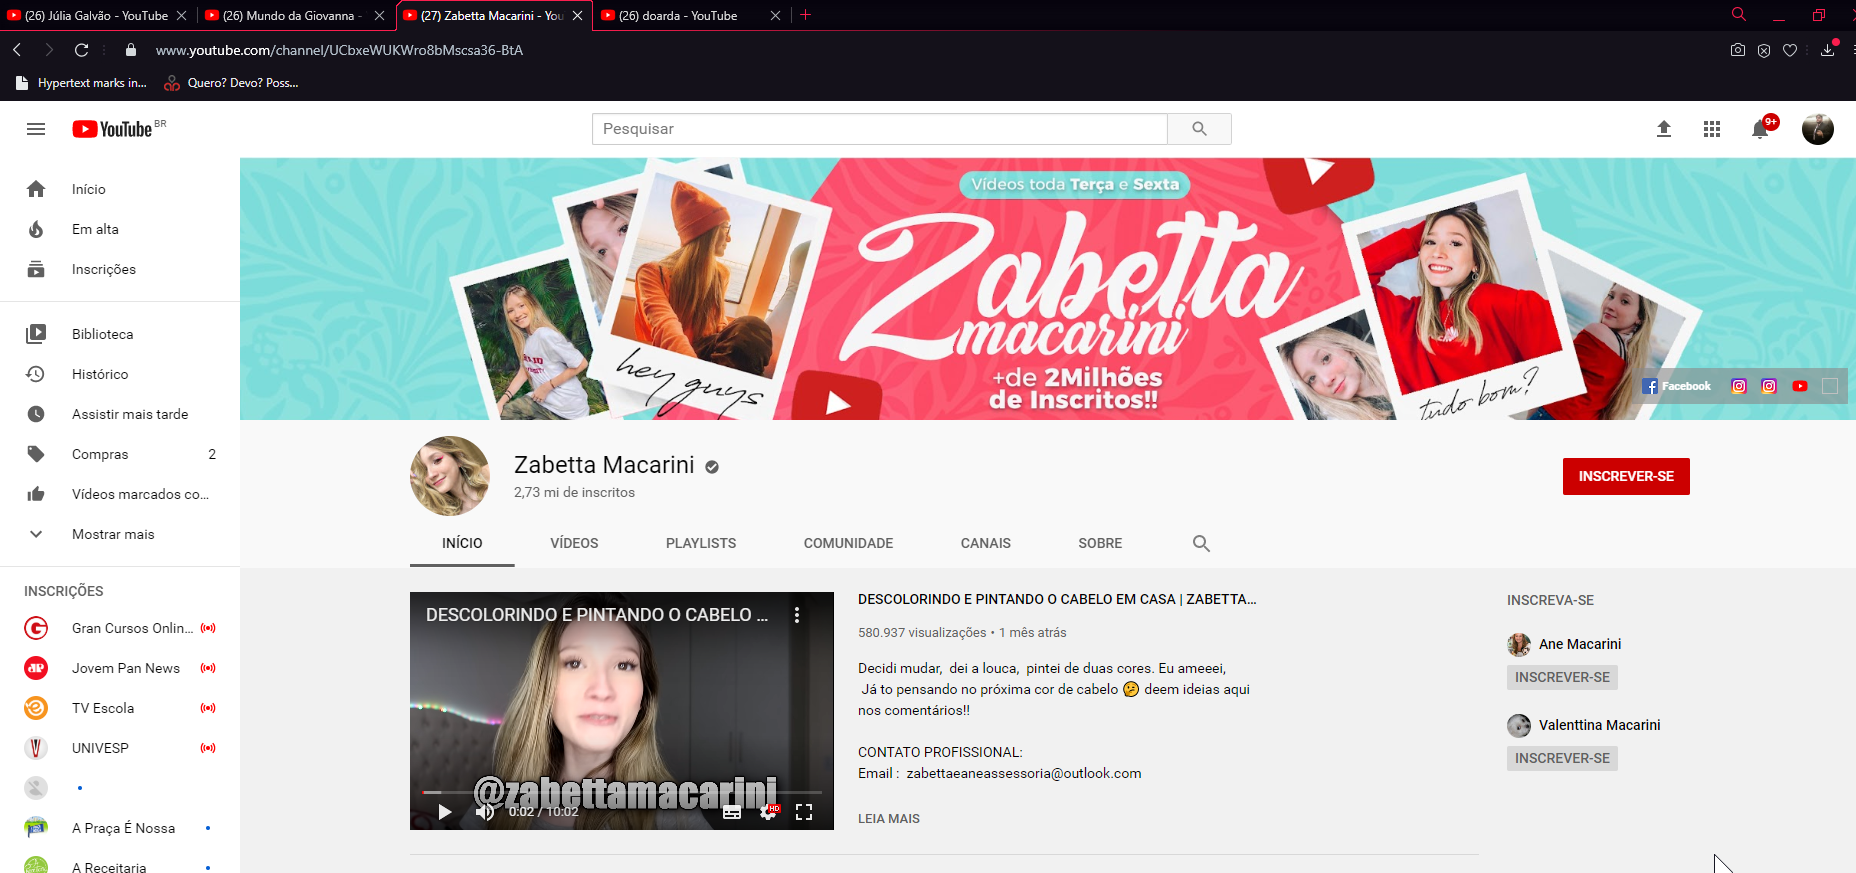
\includegraphics[width=0.999\linewidth]{fig/Canal-Zabetta-Macarini}
    }
    \caption{Tela de abertura do Canal Zabetta Macarini disponível em \url{https://www.youtube.com/channel/UCbxeWUKWro8bMscsa36-BtA}}
    \label{fig:canal-zabetta-macarini}
\end{figure}




Apresentação no OneDrive: \url{https://1drv.ms/p/s!AgRBucATAhUblzAldnG4LGnWNV-r?e=ykIvGi} \\
\begin{center}
    \href{https://1drv.ms/p/s!AgRBucATAhUblzAldnG4LGnWNV-r?e=ykIvGi}{
        \qrcode{https://1drv.ms/p/s!AgRBucATAhUblzAldnG4LGnWNV-r?e=ykIvGi}
    }
\end{center}


Vídeo no YouTube: \url{https://youtu.be/szsZ_Uuk1zk} \\
\begin{center}
    \href{https://youtu.be/szsZ_Uuk1zk}{
        \qrcode{https://youtu.be/szsZ_Uuk1zk}
    }
\end{center}
